\chapter{Project 1: VAE-Triage -- gigapixel WSI triage}

\section{Problem statement (how to pitch it)}
A pathology lab digitises hundreds of slides per day. Each WSI has $10^5$ tiles at 20$\times$. A segmentation or
classification network (U-Net, DeepLab, ViT/MIL) costs 10--100\,ms per tile on a GPU. Before spending that compute
we want to answer, \emph{per tile and on cheap hardware}: (1) is there tissue? (2) is the tile technically usable
(focus, ink, folds, exposure)? (3) what is in it (nuclei, stroma, fluid, blood, fat)? Tiles that fail (1) are dropped,
tiles that fail (2) are \emph{reported} (rescan request), and only the rest are sent to the heavy model.

\sayit{The triage gate is the cheapest place to save compute and to catch bad scans early. I built it as an
unsupervised density model so it needs no artefact annotation and runs on the scanner PC.}

\section{The original repository and what was wrong}\label{sec:bugs}
Original design: tile a TIFF with \texttt{tifffile.memmap}; train a VQ-VAE on all tiles; flag tiles whose
reconstruction MSE exceeds 0.05; export to ONNX. Problems found while reproducing it:
\begin{enumerate}
\item \textbf{Training and triage crashed.} \texttt{VQVAE.forward} returns \texttt{(x\_recon, vq\_loss, perplexity)}
but \texttt{train.py} and \texttt{triage.py} unpacked \texttt{vq\_loss, data\_recon, perplexity = model(x)}.
The ``loss'' became an image-shaped tensor and \texttt{backward()} raised
\texttt{RuntimeError: grad can be implicitly created only for scalar outputs} (reproduced). Fixed.
\item \textbf{It cannot open real WSIs.} \texttt{tifffile.memmap} works only on uncompressed contiguous TIFFs;
every scanner WSI (and every CAMELYON16 slide) is a tiled JPEG-compressed pyramid. Replaced by
\texttt{data/wsi.py}: a zarr-backed lazy reader that decodes only the TIFF tiles a request touches and exposes all
pyramid levels.
\item \textbf{Background filtering was documented but not implemented} -- every tile, including 70\% glass, went
to the network. Now a thumbnail tissue mask selects tiles.
\item \textbf{No GMM anywhere}, although the project is described as GMM-based triage. Added
\texttt{triage/gmm\_triage.py}, \texttt{triage/gmm\_components.py} and the thumbnail GMM.
\item AMP \texttt{GradScaler} was used unconditionally (warns/no-op on CPU); fixed to CUDA-only.
\item The fixed MSE threshold 0.05 is arbitrary; we calibrate thresholds as percentiles on unseen slides.
\item Synthetic ``WSI'' only (random noise + a black square) -- no evidence on real data. We benchmarked on real
CAMELYON16 slides.
\end{enumerate}

\section{Data used}
CAMELYON16 (Radboud UMC + UMC Utrecht; sentinel lymph nodes of breast-cancer patients; H\&E; 399 WSIs, 750\,GB;
AWS Open Data). We downloaded 7 slides (2 normal, 5 tumour; 4.5\,GB) with expert tumour masks and the provided
tissue/background masks. Tiles: 256$\times$256 at level 1 (20$\times$). Labels from masks: \emph{normal}
(tissue $\ge$60\%, no tumour), \emph{tumour} (tumour $\ge$60\%), \emph{background} (tissue $\le$2\%), \emph{border}.
\textbf{Split by slide}: train = normal\_108, normal\_150, tumor\_082; test = tumor\_075, 079, 084, 091.
\begin{table}[H]\centering\small
\caption{Whole-slide tile census: what Stage 0 removes before any neural network runs.}\label{tab:census}
\begin{adjustbox}{max width=\linewidth}\begin{tabular}{lrrrr}\toprule
\textbf{Slide} & \textbf{Grid tiles (256 px @20x)} & \textbf{Tissue tiles} & \textbf{Glass (skipped)} & \textbf{Tumour tiles} \\\midrule
normal\_108 & 6160 & 4279 & 30.5\% & 0 \\
normal\_150 & 15232 & 5215 & 65.8\% & 0 \\
tumor\_075 & 27104 & 11967 & 55.8\% & 312 \\
tumor\_079 & 73920 & 16389 & 77.8\% & 97 \\
tumor\_082 & 46648 & 10088 & 78.4\% & 1038 \\
tumor\_084 & 21504 & 8409 & 60.9\% & 186 \\
tumor\_091 & 12600 & 5419 & 57.0\% & 242 \\
TOTAL & 203168 & 61766 & 69.6\% & 1875 \\
\bottomrule\end{tabular}\end{adjustbox}\end{table}
\begin{figure}[H]\centering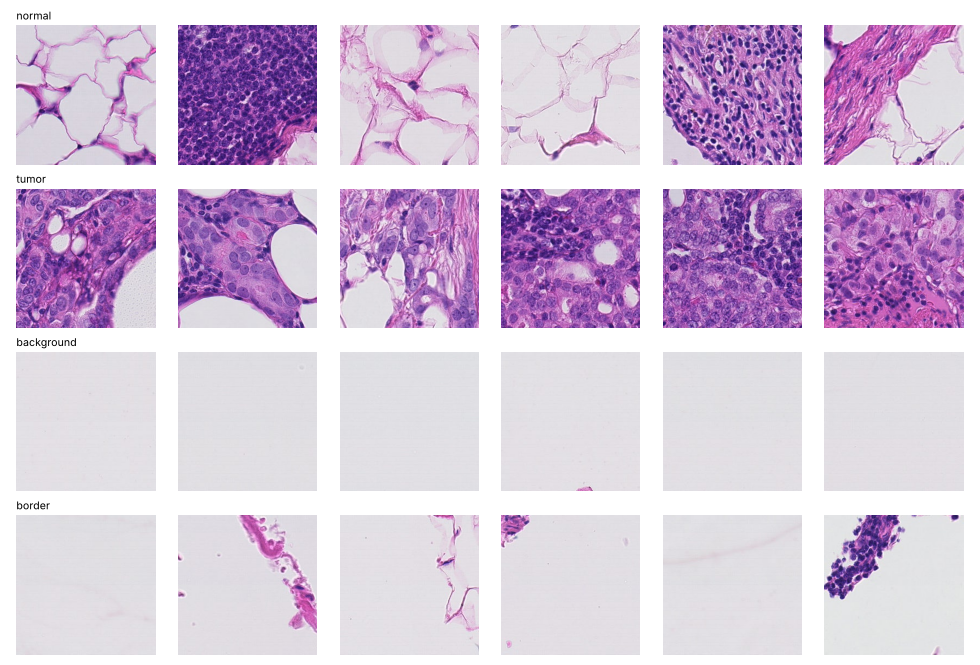
\includegraphics[width=.8\linewidth]{c16_tile_classes.png}
\caption{Real tiles: normal (note fat), tumour (metastatic carcinoma), glass, partial tissue.}\end{figure}

\paragraph{Artefact ground truth.} No public pixel-level artefact labels exist for CAMELYON16, so -- as in focus-quality
literature -- we inject 10 controlled artefacts into real clean tiles (150 each on test slides; a different random
seed on training slides is used \emph{only} by supervised baselines): Gaussian blur ($\sigma$=1.5--4), motion blur
(9--25\,px), partial blur, pen ink, tissue fold (Beer--Lambert 2--3$\times$ OD), air bubble, washout, dark exposure,
sensor noise, JPEG (q=3--10).
\begin{figure}[H]\centering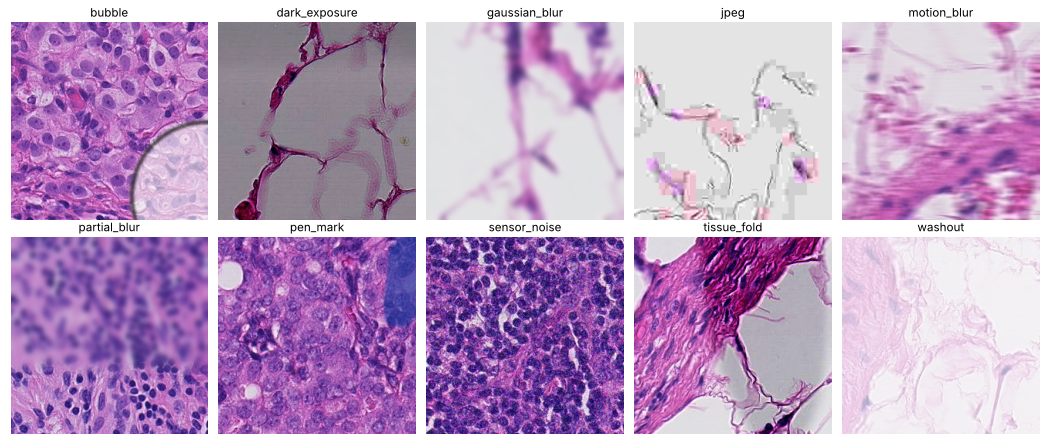
\includegraphics[width=.9\linewidth]{c16_artifacts.png}\caption{The 10 artefact simulators.}\end{figure}

\section{Stage 0 -- thumbnail tissue detection}
On a $\sim$4--8\,$\mu$m/px thumbnail we compare thresholding, k-means and a 2-component GMM on (HSV saturation,
optical density), with morphological opening/closing and small-component removal (scanner stripes and dust).
\begin{table}[H]\centering\small
\caption{Stage-0 tissue detection on 7 CAMELYON16 slides (mean over slides).}\label{tab:tissue}
\begin{adjustbox}{max width=\linewidth}\begin{tabular}{lrrrr}\toprule
\textbf{Method (thumbnail, ~4-8 um/px)} & \textbf{Dice} & \textbf{IoU} & \textbf{Precision} & \textbf{Recall} \\\midrule
Fixed threshold (gray < 220) & 0.743 & 0.604 & 0.890 & 0.669 \\
Otsu on grayscale & 0.522 & 0.364 & 0.986 & 0.365 \\
Otsu on HSV saturation & 0.552 & 0.398 & 0.999 & 0.398 \\
Otsu on saturation + morphology & 0.534 & 0.381 & 0.999 & 0.381 \\
K-means (k=2) on (S, OD) & 0.138 & 0.078 & 0.982 & 0.079 \\
GMM (K=2) on (S, OD) + morphology {[}ours{]} & 0.839 & 0.746 & 0.929 & 0.805 \\
\bottomrule\end{tabular}\end{adjustbox}\end{table}
\begin{figure}[H]\centering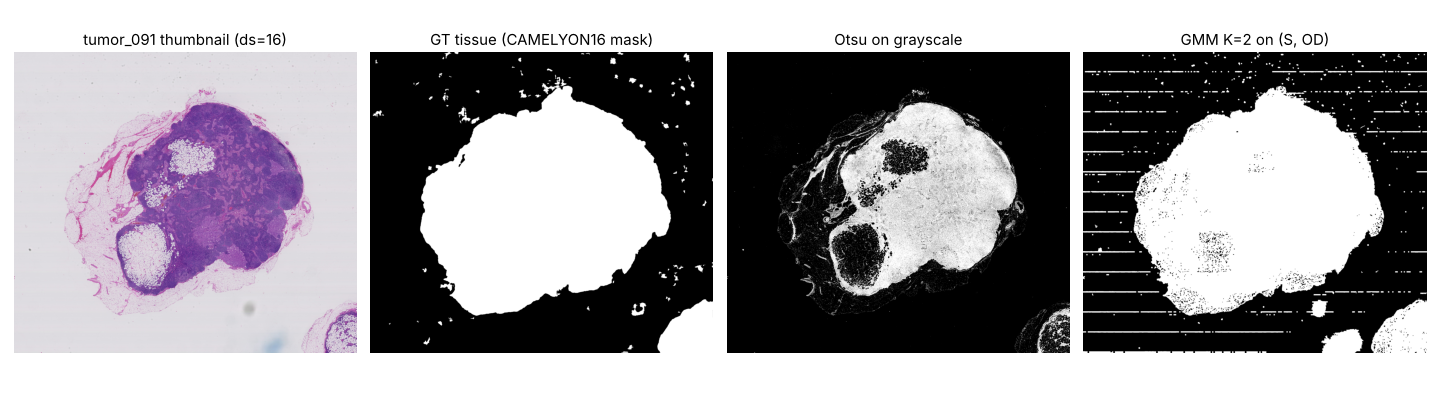
\includegraphics[width=\linewidth]{tissue_detection_tumor_091.png}
\caption{Otsu misses faint fat/loose tissue (it assumes two equally spread classes); the GMM captures the broad
tissue cluster. Remaining GMM errors: scanner stripes in glass (removed by opening) and the perinodal fat that the
reference mask excludes.}\end{figure}
\keyidea{Glass is a tight cluster, tissue a broad one. A GMM models unequal variances and priors; Otsu and k-means do
not. Dice 0.84 vs 0.53 (Otsu) vs 0.14 (k-means).}

\section{Stage 1 -- tile QC with a GMM density}
\subsection{Features (23, all physically motivated)}
Tissue: tissue fraction, white fraction, dark fraction. Stain: mean/std of OD, of H and E concentrations (colour
deconvolution), saturation/value statistics, non-H\&E-hue fraction (pen ink), colourfulness. Focus: log Laplacian
variance, log Tenengrad, log Brenner, contrast-normalised Laplacian, FFT high-frequency ratio. Structure: Canny edge
density, grey-level entropy. Noise: residual vs median filter. Cost: $\sim$5\,ms per 256$^2$ tile (one core).

\subsection{Model and calibration}
Robust standardisation (median/IQR) $\to$ full-covariance GMM fitted by EM on clean training tiles, $K$ chosen by
held-out-slide log-likelihood; score $-\log p(\mathbf{x})$; threshold = 95th percentile of scores on \emph{unseen}
training slides (leave-one-slide-out). The exported model is a 45\,KB JSON (means, Cholesky factors of precisions,
weights) scored by NumPy in 0.01\,ms/tile.

\subsection{Results}
\begin{table}[H]\centering\small
\caption{Stage-1 tile QC on 4 unseen test slides: 2290 clean tissue tiles vs. 600 glass + 1500 artefact tiles. Unsupervised thresholds calibrated on unseen training slides (95\% clean pass).}\label{tab:qc}
\begin{adjustbox}{max width=\linewidth}\begin{tabular}{>{\raggedright\arraybackslash}p{6.8cm}rrrrrrr}\toprule
\textbf{Method} & \textbf{AUROC} & \textbf{AUPRC} & \textbf{Prec.} & \textbf{Recall} & \textbf{F1} & \textbf{Spec.} & \textbf{Tum. rej.} \\\midrule
Tissue fraction (Otsu-like) & 0.609 & 0.690 & 0.833 & 0.348 & 0.491 & 0.936 & 0.004 \\
Laplacian variance (focus) & 0.759 & 0.794 & 0.874 & 0.537 & 0.665 & 0.929 & 0.004 \\
Tenengrad (Sobel energy) & 0.764 & 0.792 & 0.847 & 0.494 & 0.624 & 0.918 & 0.004 \\
HistoQC-style rule set & 0.857 & 0.861 & 0.936 & 0.463 & 0.620 & 0.971 & 0.004 \\
Single Gaussian (Mahalanobis, K=1) & 0.954 & 0.943 & 0.923 & 0.890 & 0.906 & 0.932 & 0.006 \\
GMM (K=4) same-slide calibration {[}pitfall{]} & 0.942 & 0.936 & 0.735 & 0.948 & 0.828 & 0.687 & 0.431 \\
GMM (K=6, BIC) LOSO calibration {[}ours{]} & 0.939 & 0.933 & 0.894 & 0.892 & 0.893 & 0.903 & 0.084 \\
GMM (K=6, slide-CV) LOSO calibration {[}ours, final{]} & 0.939 & 0.933 & 0.918 & 0.876 & 0.897 & 0.928 & 0.035 \\
GMM on QC-only feature subset {[}ours, tumour-safe{]} & 0.937 & 0.928 & 0.944 & 0.721 & 0.818 & 0.961 & 0.002 \\
Isolation Forest & 0.913 & 0.876 & 0.899 & 0.690 & 0.780 & 0.929 & 0.004 \\
One-class SVM (RBF) & 0.905 & 0.904 & 0.938 & 0.658 & 0.773 & 0.960 & 0.006 \\
Logistic regression (supervised) & 0.966 & 0.949 & 0.925 & 0.927 & 0.926 & 0.931 & 0.004 \\
Random forest (supervised) & 0.960 & 0.955 & 0.863 & 0.930 & 0.895 & 0.865 & 0.020 \\
VQ-VAE recon-MSE (LOSO-calibrated threshold) & 0.376 & 0.517 & 0.736 & 0.178 & 0.286 & 0.941 & 0.020 \\
VQ-VAE recon-MSE (repo default threshold 0.05) & 0.376 & 0.517 & 0.582 & 0.207 & 0.305 & 0.863 & 0.129 \\
ResNet18-ImageNet feats + PCA32 + GMM(K=4) & 0.769 & 0.708 & 0.714 & 0.197 & 0.309 & 0.928 & 0.043 \\
MobileNetV3-Small supervised QC & 0.976 & 0.958 & 0.876 & 0.982 & 0.926 & 0.873 & 0.051 \\
\bottomrule\end{tabular}\end{adjustbox}\end{table}
\begin{figure}[H]\centering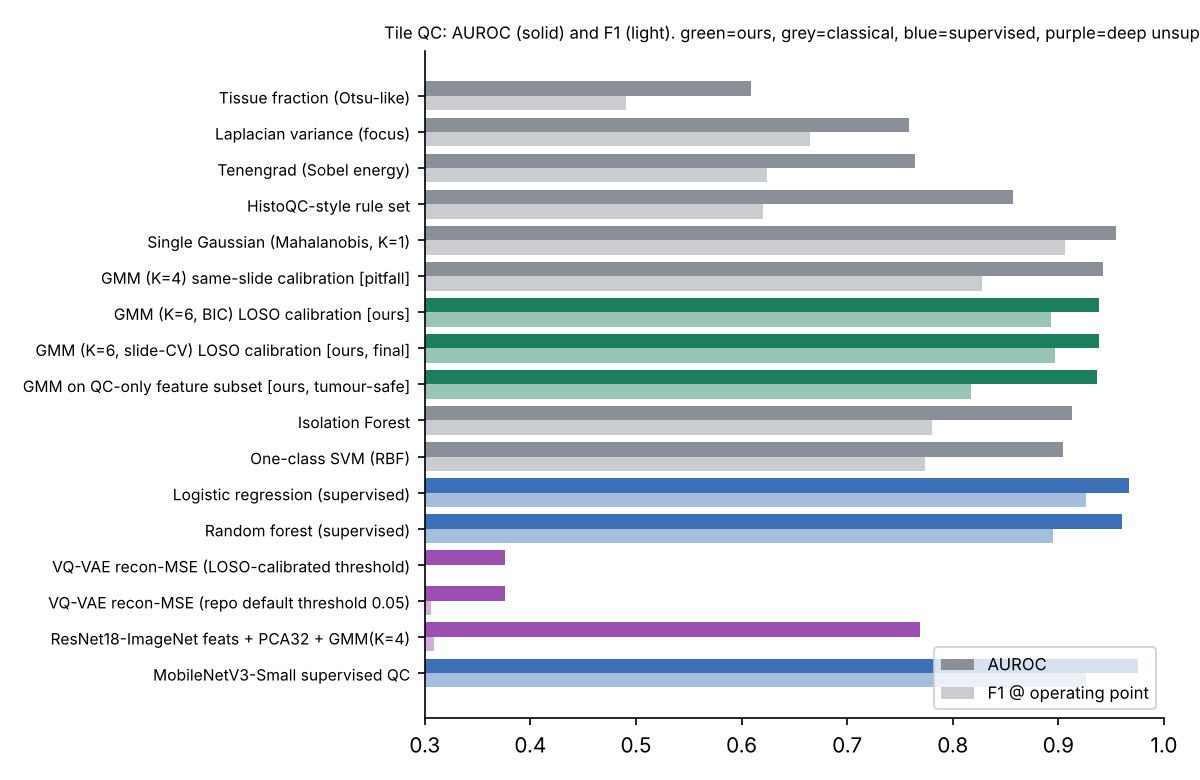
\includegraphics[width=.9\linewidth]{chart_qc.png}\caption{QC methods, test slides.}\end{figure}
\begin{figure}[H]\centering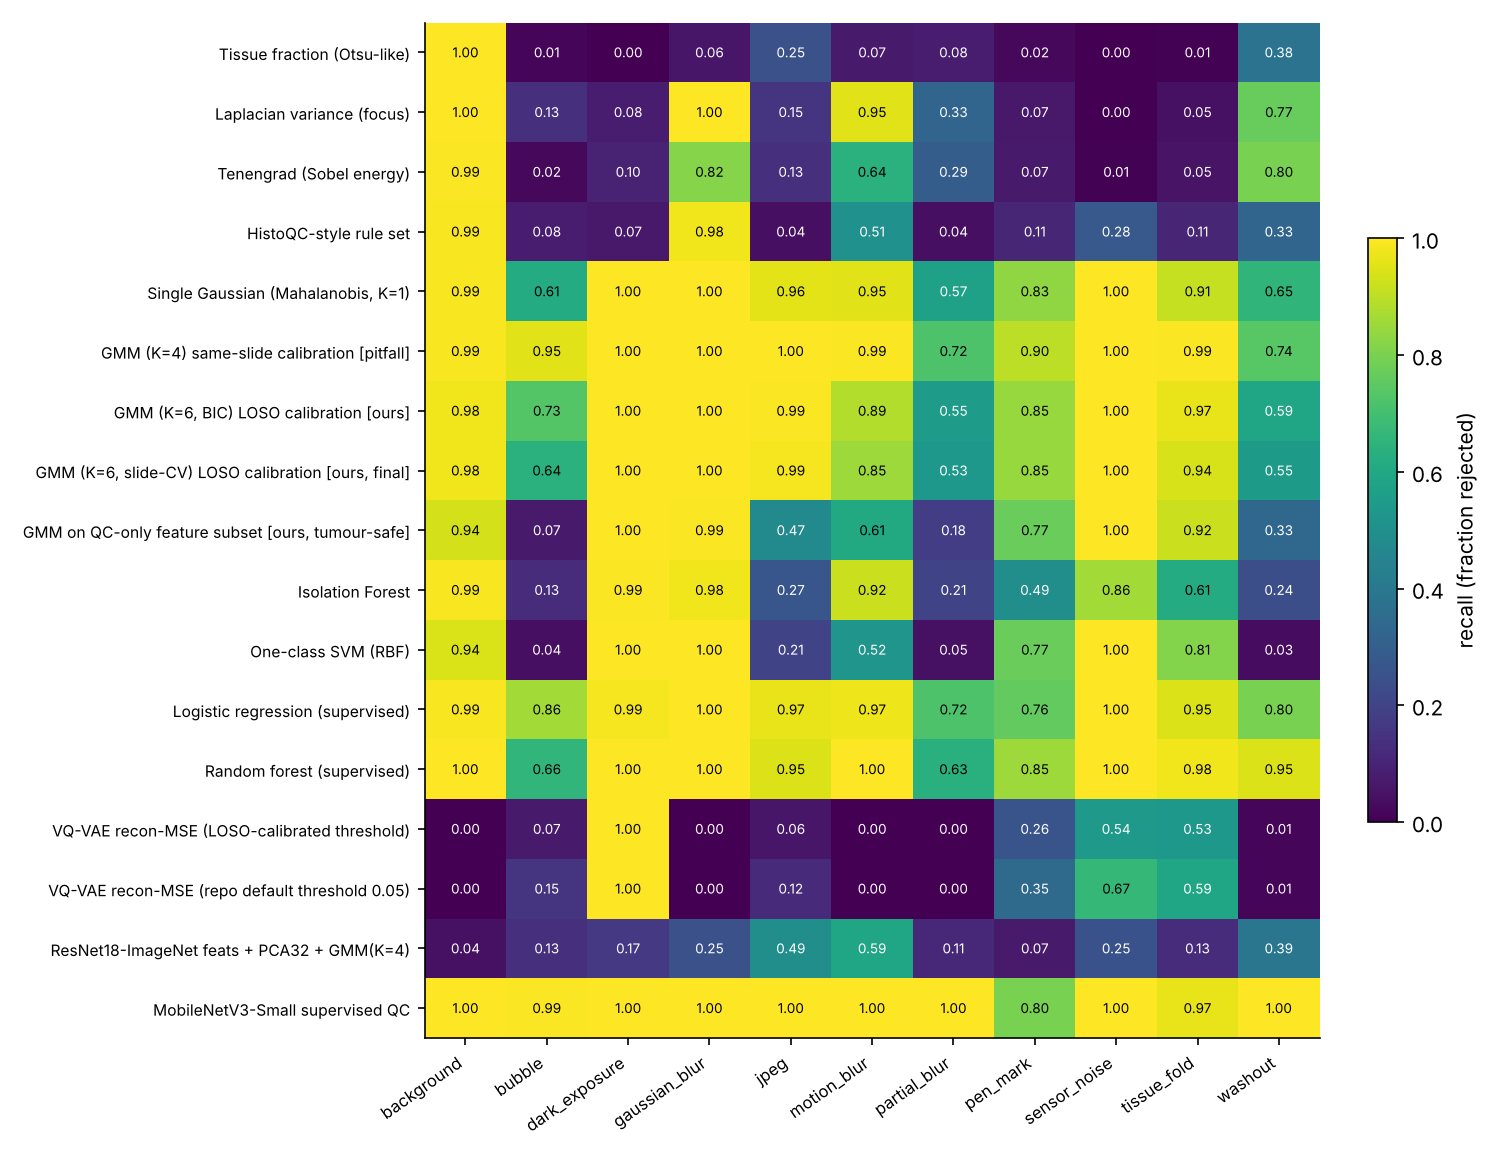
\includegraphics[width=\linewidth]{chart_qc_per_artifact.png}
\caption{Recall per artefact at the operating point. Single-cue methods catch one artefact family each
(Laplacian: blur; tissue fraction: glass); the density models catch nearly all; partial blur, bubbles and washout
are hardest.}\end{figure}
\begin{figure}[H]\centering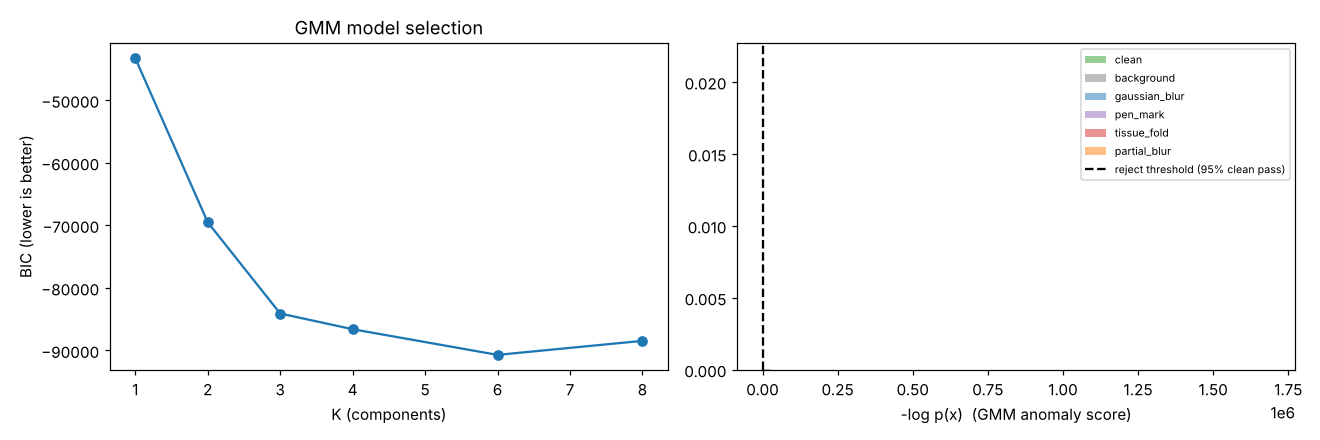
\includegraphics[width=\linewidth]{gmm_bic_and_scores.png}
\caption{Left: BIC keeps decreasing with $K$ because tiles are correlated within a slide (BIC assumes i.i.d.).
Right: GMM score distributions; the dashed line is the reject threshold.}\end{figure}

\paragraph{Interpretation.}
\begin{itemize}
\item \textbf{The original VQ-VAE score is the wrong tool for QC: AUROC 0.376 (worse than chance).} Blurred, washed-out and
empty tiles are \emph{smooth}, and smooth images are the easiest to reconstruct, so their MSE is \emph{lower} than that of
sharp, textured tissue. With the repo's fixed threshold 0.05 it catches 21\% of artefacts. This is the most important
finding to understand and to say honestly.
\item Supervised MobileNetV3-Small (fine-tuned on our synthetic artefacts) is the best QC model (AUROC 0.976, F1 0.926,
0.6\,ms/tile in ONNX Runtime) -- \emph{but only for artefact types it was trained on} (Table~\ref{tab:unseen}).
\item Density models on hand-crafted features (single Gaussian 0.954, GMM 0.939 AUROC) are within 1--3 points of
\emph{supervised} classifiers (0.96--0.97) that need artefact labels -- and far above single-cue rules (0.61--0.86).
\item A single Gaussian is as good as the mixture here: with 3 training slides, extra components fit
slide-specific appearance. Say this openly -- it shows understanding of the bias/variance trade-off.
\item \textbf{Calibration trap.} Thresholding on held-out tiles of the \emph{same} slides gives specificity 0.69 and
rejects 43\% of tumour tiles on new slides; calibrating on unseen slides gives 0.93 specificity and 3.5\% tumour
rejection. Tumour looks ``unusual'' to a model of mostly-normal tissue, so a QC gate must be checked for this failure.
\item \textbf{Explainability}: the GMM decomposes a rejection into z-scores. Examples from our run: Gaussian blur
$\to$ \texttt{lap\_norm} $-10.5\sigma$, \texttt{log\_lap\_var} $-9.9\sigma$; tissue fold $\to$ \texttt{dark\_frac}
$+31\sigma$; glass $\to$ \texttt{log\_tenengrad} $-7.4\sigma$.
\item A tumour-safe variant (GMM on 14 QC-only features, no morphology/stain-pattern features) rejects only 0.2\% of
tumour but recall drops to 0.72 -- a deployment knob.
\end{itemize}
\begin{table}[H]\centering\small
\caption{Which features move most under each artefact (Jensen-Shannon divergence, base 2, in [0,1]).}\label{tab:js}
\begin{adjustbox}{max width=\linewidth}\begin{tabular}{lp{11cm}}\toprule
\textbf{Artefact} & \textbf{Top-3 features by JS divergence (clean vs artefact)} \\\midrule
background & colorfulness (0.95), tissue\_frac (0.94), sat\_std (0.93) \\
bubble & hf\_ratio (0.35), h\_std (0.31), lap\_norm (0.29) \\
dark\_exposure & val\_mean (0.94), tissue\_frac (0.80), h\_mean (0.56) \\
gaussian\_blur & lap\_norm (0.94), log\_lap\_var (0.91), log\_noise (0.90) \\
jpeg & dark\_frac (0.31), log\_noise (0.27), edge\_density (0.23) \\
motion\_blur & log\_lap\_var (0.82), lap\_norm (0.79), hf\_ratio (0.66) \\
partial\_blur & log\_noise (0.37), edge\_density (0.36), log\_lap\_var (0.32) \\
pen\_mark & non\_he\_hue\_frac (0.31), h\_mean (0.22), h\_std (0.22) \\
sensor\_noise & non\_he\_hue\_frac (0.94), log\_noise (0.76), colorfulness (0.43) \\
tissue\_fold & dark\_frac (0.46), od\_std (0.36), val\_std (0.35) \\
washout & e\_std (0.78), sat\_std (0.76), od\_std (0.69) \\
\bottomrule\end{tabular}\end{adjustbox}\end{table}
\begin{figure}[H]\centering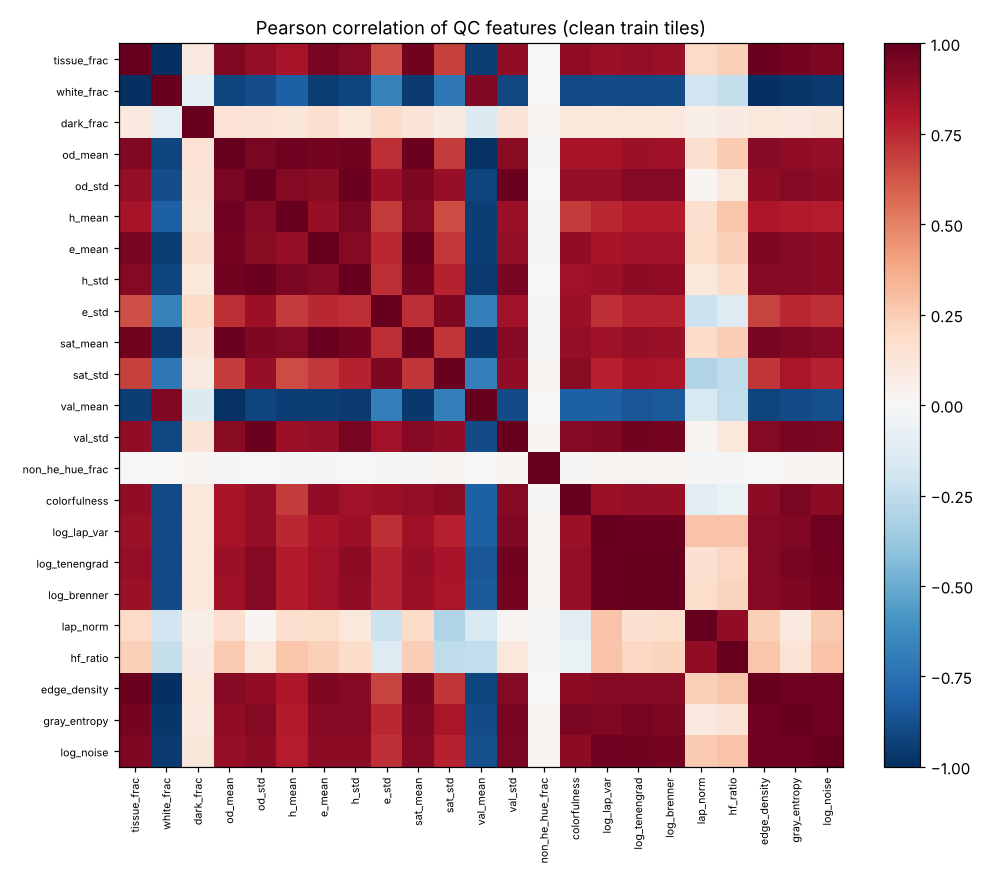
\includegraphics[width=.48\linewidth]{feature_correlation.png}\hfill
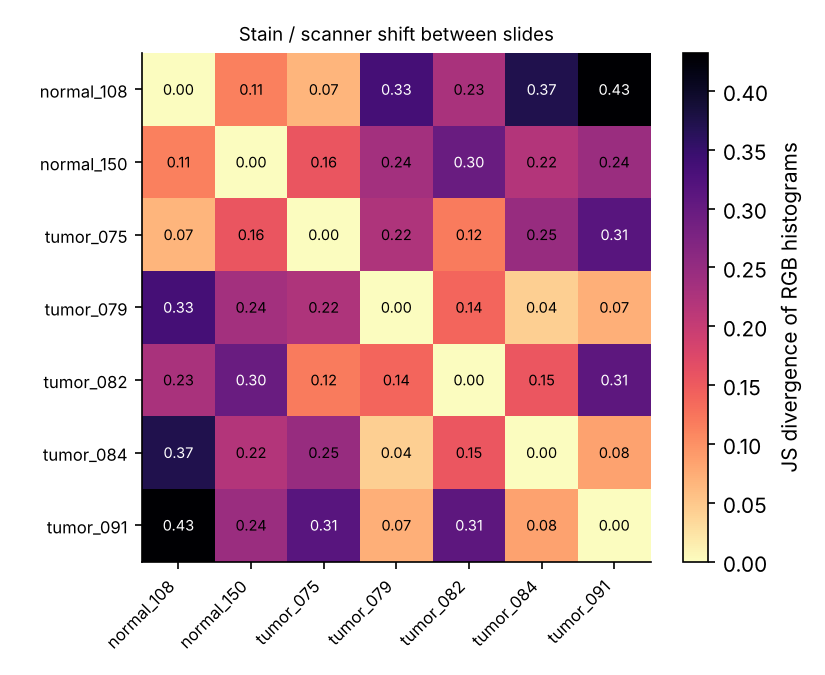
\includegraphics[width=.48\linewidth]{chart_slide_js.png}
\caption{Left: feature correlations (tissue-amount and focus features are strongly correlated; 4 principal directions
hold 90\% of variance). Right: JS divergence of RGB histograms between slides = stain/scanner shift.}\label{fig:slidejs}\end{figure}

\subsection{Why unsupervised: artefacts never seen in training}
\begin{table}[H]\centering\small
\caption{Recall on artefact types NEVER seen in training (supervised models saw the other 6 types).}\label{tab:unseen}
\begin{adjustbox}{max width=\linewidth}\begin{tabular}{p{7cm}rrrrr}\toprule
\textbf{Model} & \textbf{bubble} & \textbf{pen ink} & \textbf{fold} & \textbf{JPEG} & \textbf{clean rejected} \\\midrule
Logistic regression (supervised, 6 artefact types seen) & 0.13 & 0.64 & 0.41 & 0.46 & 0.041 \\
Random forest (supervised, 6 artefact types seen) & 0.07 & 0.64 & 0.24 & 0.22 & 0.062 \\
GMM K=1 (no artefact ever seen) & 0.61 & 0.83 & 0.91 & 0.96 & 0.068 \\
GMM K=6 (no artefact ever seen) & 0.64 & 0.85 & 0.94 & 0.99 & 0.072 \\
\bottomrule\end{tabular}\end{adjustbox}\end{table}
Supervised classifiers trained on 6 artefact types catch only 7--64\% of the 4 held-out types; the GMM, which never saw
any artefact, catches 64--99\% at a similar clean-rejection rate. A scanner in production will produce artefacts no one
annotated -- novelty detection is the right formulation for QC; supervised models are the right tool once a failure mode
is known and labelled. \textbf{Best design: GMM gate for the unknown + small supervised head for known, frequent artefacts.}

\section{Stage 2 -- GMM tissue components and fluid separation}\label{sec:fluid}
Per-pixel descriptor $[C_H, C_E, \mathrm{OD}, a^*, \text{local std}]$; full-covariance GMM with $K=7$ fitted on
200k pixels from 120 training tiles (40\,s), components named by rules on their means: OD$<0.2$ background/fat;
$C_H/(C_H+C_E)>0.6$ nuclei; $a^*>0.45$ and $C_E>C_H$ blood; $0.2\le$OD$<0.45$ and $C_E\ge C_H$ \textbf{fluid}
(pale, eosinophilic: proteinaceous fluid, plasma, oedema, lymph); else stroma/cytoplasm.
\begin{figure}[H]\centering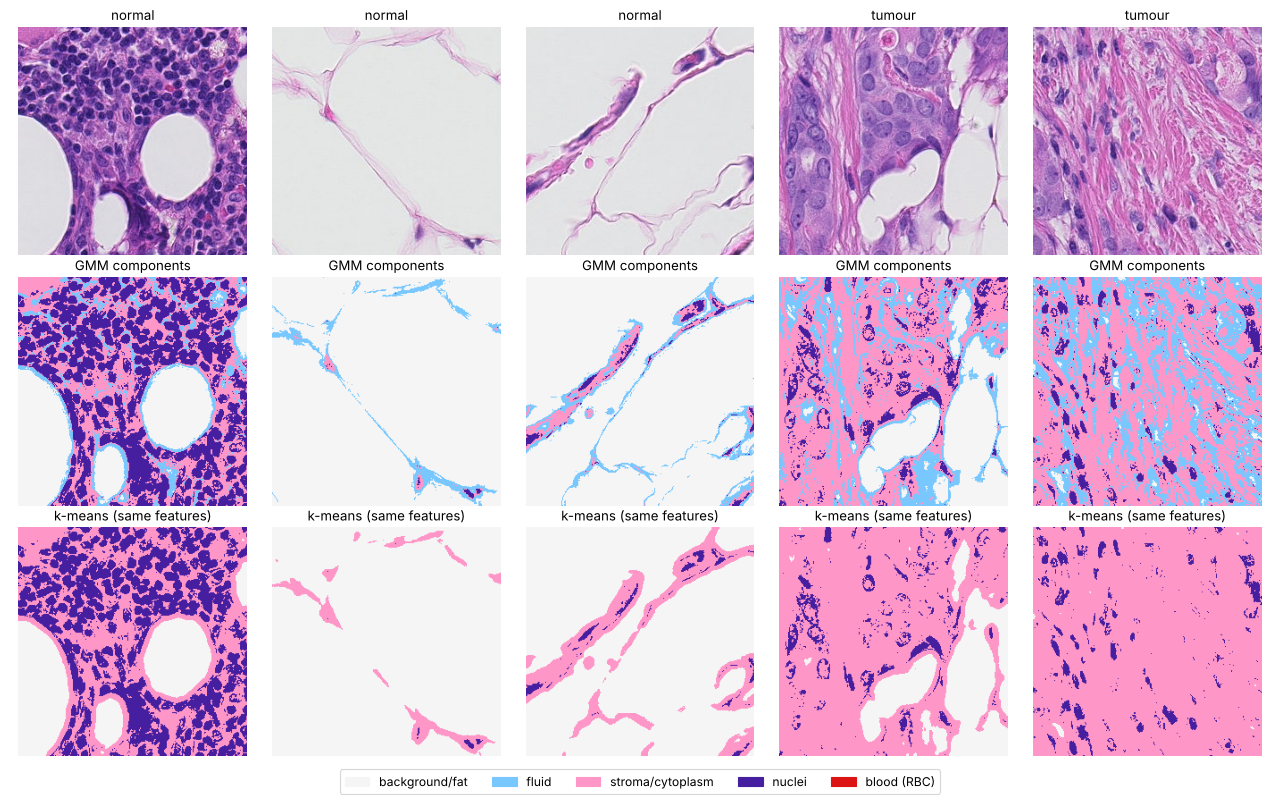
\includegraphics[width=\linewidth]{gmm_tissue_components.png}
\caption{GMM components vs k-means on the same 5-D descriptor. The GMM isolates a pale eosinophilic (fluid)
component around fat septa and in loose tissue; k-means merges it into stroma.}\end{figure}
\begin{table}[H]\centering\small
\caption{Mean GMM component fractions per tile (test slides).}\label{tab:components}
\begin{adjustbox}{max width=\linewidth}\begin{tabular}{lrrrr}\toprule
\textbf{Tile class} & \textbf{Background/fat} & \textbf{Fluid} & \textbf{Stroma/cytoplasm} & \textbf{Nuclei} \\\midrule
normal & 0.525 & 0.107 & 0.177 & 0.191 \\
tumor & 0.072 & 0.150 & 0.501 & 0.277 \\
\bottomrule\end{tabular}\end{adjustbox}\end{table}
\paragraph{Quantitative checks (no pixel labels exist for fluid).} (1) Stability: two GMMs fitted on disjoint slides
agree on 79\% of pixels (ARI 0.68). (2) k-means on the same features finds no fluid cluster. (3) Usefulness:
the 5 component fractions alone separate tumour from normal tiles with \textbf{AUROC 0.931} (logistic regression on
train-slide labels); stroma/cytoplasm fraction alone gives 0.928. Tumour tiles have 2.8$\times$ more stroma/cytoplasm
and far less fat. Cost: 85\,ms per 256$^2$ tile at full resolution, $\sim$5\,ms when run on a 4$\times$ downsampled tile.
\warn{The pale-eosinophilic class also contains loose connective tissue and pale cytoplasm edges -- colour alone cannot
fully separate them. Say: ``the GMM gives a fluid-likelihood map; for a clinical fluid quantification I would refine it
with texture (fluid is homogeneous) or a small supervised model trained on a few annotated regions''.}

\section{Tumour triage (anomaly detection) and the deep baselines}
\begin{table}[H]\centering\small
\caption{Tumour (metastasis) vs. normal tiles on test slides (490 tumour / 1800 normal). Literature rows use different splits and are indicative only.}\label{tab:tumour}
\begin{adjustbox}{max width=\linewidth}\begin{tabular}{p{8.2cm}rrl}\toprule
\textbf{Method} & \textbf{AUROC} & \textbf{AUPRC} & \textbf{Type} \\\midrule
GMM novelty (K=4) on features & 0.740 & 0.318 & unsup. \\
Isolation Forest on features & 0.661 & 0.257 & unsup. \\
Hematoxylin mean (single feature) & 0.711 & 0.290 & unsup. \\
Logistic regression (supervised) & 0.890 & 0.586 & sup. \\
Random forest (supervised) & 0.945 & 0.797 & sup. \\
VQ-VAE recon-MSE novelty (trained on normal) & 0.749 & 0.317 & unsup. \\
ResNet18 feats + GMM novelty (trained on normal) & 0.671 & 0.272 & unsup. \\
MobileNetV3-Small supervised (1 tumour slide) & 0.557 & 0.436 & sup. \\
GMM tissue-component fractions + LR {[}ours{]} & 0.931 & -- & unsup. feats + sup. LR \\
\midrule
Lit: L1 autoencoder, unsup. (Shvetsova'21) & 0.211 & -- & literature \\
Lit: AE (cross-organ, AnoPILaD'25) & 0.658 & -- & literature \\
Lit: AnoDDPM diffusion (AnoPILaD'25) & 0.686 & -- & literature \\
Lit: Deep-IF ImageNet feats (Shvetsova'21) & 0.906 & -- & literature \\
Lit: Deep perceptual AE (Shvetsova'21) & 0.934 & -- & literature \\
\bottomrule\end{tabular}\end{adjustbox}\end{table}
\begin{figure}[H]\centering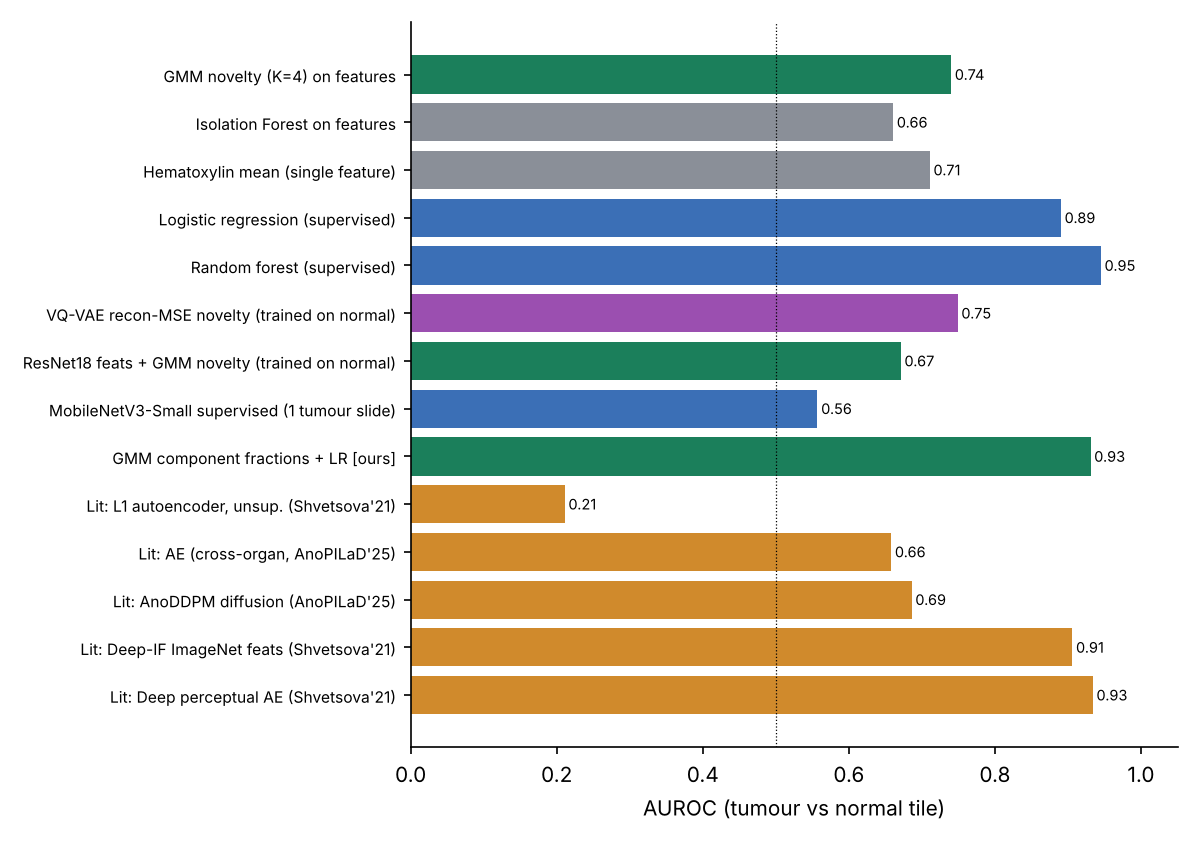
\includegraphics[width=.9\linewidth]{chart_tumour.png}
\caption{Tumour vs normal tiles. Orange = literature (different splits, indicative).}\end{figure}
Reading the table: unsupervised novelty scores reach 0.67--0.75 (GMM on QC features 0.740, VQ-VAE reconstruction 0.749,
ImageNet-ResNet features + GMM 0.671) -- in line with reconstruction autoencoders in the literature (0.66) and far from
supervised models. Tissue-component fractions (0.93) and a random forest on features (0.945) are best. The supervised
MobileNetV3 trained on tumour tiles from \emph{one} slide reaches only 0.557: with one training slide a CNN memorises that
slide's stain -- the classic reason why pathology models need many slides from many centres plus stain augmentation.

\section{Edge cost}
\begin{table}[H]\centering\small
\caption{Measured inference cost on this 4-vCPU cloud container (no GPU).}\label{tab:latency}
\begin{adjustbox}{max width=\linewidth}\begin{tabular}{p{6cm}rp{4cm}l}\toprule
\textbf{Component} & \textbf{ms / 256px tile} & \textbf{Model size} & \textbf{Hardware} \\\midrule
Hand-crafted features (23-D, NumPy/OpenCV) & 5.0 & 0 (no weights) & CPU, 1 core \\
GMM scorer (NumPy, JSON params) & 0.0093 & 45 KB JSON (1799 params) & CPU \\
VQ-VAE PyTorch FP32 & 37.21 & 0.69 M params & CPU, 4 threads \\
VQ-VAE ONNX Runtime FP32 & 22.88 & 2.9 MB & CPU, 4 threads \\
VQ-VAE ONNX Runtime INT8 & 22.74 & 0.8 MB & CPU, 4 threads \\
MobileNetV3-S ONNX Runtime FP32 & 0.60 & 6.1 MB & CPU, 4 threads \\
MobileNetV3-S ONNX Runtime INT8 & 1.39 & 1.7 MB & CPU, 4 threads \\
ResNet-18 features PyTorch FP32 & 15.83 &  & CPU, 4 threads \\
\bottomrule\end{tabular}\end{adjustbox}\end{table}
\begin{figure}[H]\centering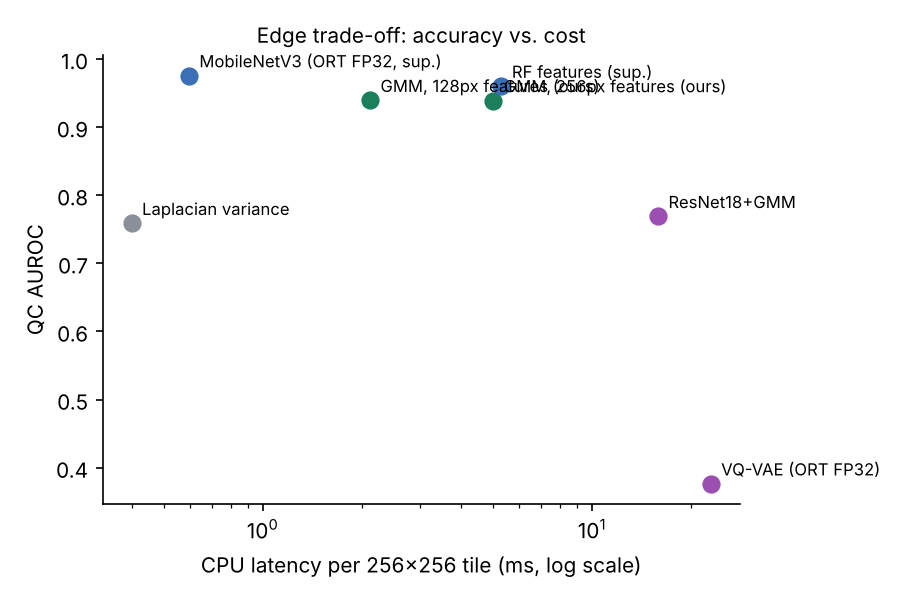
\includegraphics[width=.6\linewidth]{chart_edge_tradeoff.png}\caption{Accuracy vs cost.}\end{figure}
\begin{table}[H]\centering\small
\caption{Edge optimisation: features on a 2x-downsampled tile.}\label{tab:downsample}
\begin{adjustbox}{max width=\linewidth}\begin{tabular}{p{8cm}rr}\toprule
\textbf{Variant} & \textbf{feature ms/tile} & \textbf{QC AUROC} \\\midrule
Full-res features (256 px), GMM K=6 & 5.0 & 0.939 \\
Features on 128 px (2x down), GMM K=1 & 2.1 & 0.950 \\
Features on 128 px (2x down), GMM K=6 & 2.1 & 0.939 \\
\bottomrule\end{tabular}\end{adjustbox}\end{table}
\paragraph{Honest edge comparison.} The GMM itself costs 0.01\,ms; the hand-crafted features dominate (5\,ms at 256\,px,
2.1\,ms at 128\,px with no AUROC loss). A MobileNetV3-Small in ONNX Runtime runs at 0.6\,ms/tile on 4 threads -- so on
a multi-core CPU a tiny CNN is not slower. The GMM's real edge advantages are: no labels, no training data for each new
artefact, 45\,KB model with no runtime dependency, interpretability, and graceful handling of unseen failures.
INT8 static quantisation shrank the ONNX models 3.5--3.7$\times$ (VQ-VAE 2.9$\to$0.8\,MB, rank correlation of scores
0.988) but did \emph{not} speed them up on this CPU (VQ-VAE 22.9$\to$22.7\,ms; MobileNet 0.6$\to$1.4\,ms because of
quantise/dequantise overhead without VNNI kernels) -- always measure on the target device.
\paragraph{Whole-slide arithmetic.} A typical slide here has 29{,}000 grid tiles; Stage 0 keeps $\sim$8{,}800.
Features (128\,px) + GMM: 8{,}800 $\times$ 2.1\,ms $\approx$ 18\,s on one core, $\sim$5\,s on 4 cores, no GPU. The heavy model then
processes 30\% of the grid instead of 100\%.
